\documentclass[letterpaper]{article}
\usepackage{aaai}
\usepackage{times}
\usepackage{helvet}
\usepackage{courier}
\usepackage{graphicx}
\usepackage{subcaption}

\frenchspacing
\setlength{\pdfpagewidth}{8.5in}
\setlength{\pdfpageheight}{11in}

\pdfinfo{
/Title Distance Based Guidance of Goal Trajectories
/Subject AAAI-16 Doctoral Consortium Thesis Abstract
/Author Benjamin Bengfort, Michael T. Cox}

\title{Distance Based Guidance of Goal Trajectories}
\author{Benjamin Bengfort\\
Department of Computer Science\\
University of Maryland\\
\textit{bengfort@cs.umd.edu}\\
\And
Michael T. Cox\\
UMD Institute for Advanced Computer Studies\\
Wright State Research Institute\\
\textit{michael.cox@wright.edu}
}

\setcounter{secnumdepth}{0}
\nocopyright

\begin{document}

    \maketitle

\begin{abstract}
Mixed initiative knowledge-goal reasoning systems augment human information retrieval and investigation by providing guidance in order to accelerate the amount of time it takes to solve a knowledge goal. Guidance is provided by a cognitive system that reasons about the high level goals of the user through a case based learning mechanism. As the cognitive system gains more experience and therefore more cases, it is able to detect similarity in knowledge goals and prompt the user with additional relevant goals that short circuit or short cut the human reasoning process to minimize tangents or false starts. In this paper we present a distance-based guidance mechanism that reduces the total length of a goal trajectory through guidance that accelerates the human reasoning process.
\end{abstract}

\section{Introduction}

Information retrieval systems using statistical inference mechanisms have changed the way we interact with data. Search techniques have evolved to allow the parsing of natural language questions into a structured database query \cite{yahya_natural_2012} or lambda calculus representation \cite{berant_semantic_2013} that can executed against a structured knowledge base. This has resulted in a shift in the balance between the amount of work a human has to do to solve a \textit{knowledge goal} and the amount of work of the cognitive augmentation system. For example previous search techniques were designed to deliver the most relevant content to the human user, but left them the task of reading and interpreting that content to inform their specific goals.

Now, because human users can get immediate, automated responses to fact oriented questions including superlative and aggregation questions (e.g. ``which country has the most gold medals per capita?'') the focus has shifted to higher level goals, particularly those that require creativity like \textit{explaination} or \textit{assosciative} knowledge goals. These types of knowledge goals require a research or investigative approach to reasoning, where an initial knowledge goal changes throughout the course of solving the goal because of new information and increasing precision. Therefore we can say that the act of investigation necessarily involves the creation of a \textit{knowledge goal trajectory}, where the posing of an initial knowledge goal is refined, focused, or changed through a variety of phases in the investigative sequence, usually in a creative manner as a reaction to information retrieved with factual sub-knowledge goals that can be quickly retrieved to confirm or reject hypotheses or assumptions that led to the initial goal.

Because of the creative elements of this type of reasoning, crowd-sourcing has become a popular approach for investigation \cite{wang_wisdom_2013}. Instead, we propose a mixed-initiaitve interactive knowledge-goal reasoning system where humans propose their investigations in the form of \textit{dialogues} -- a discrete interval or set of questions posed to the system with associated retrievals. The underlying reasoning system leverages a case based approach to provide \textit{guidance} to the user such that the investigative process is short circuited or accelerated. By representing knowledge goals as a multi-dimensional vector of semantic features, we can compute the distance between knowledge goals in goal space. As users interact with the system, the total goal distance can be computed as the length of the path of knowledge goals from the initial to final goals of the dialogue. If a system is able to recommend goals by reusing previous cases that decrease the length of the goal trajectory, or simply short circuit tangents or bad investigative paths, then it can be said to be providing guidance and augmenting the cognitive aspects of investigation for a human user.

Our approach builds upon previous work \cite{bengfort_interactive_2015}, particularly a taxonomy of knowledge goals, in order to create a multi-dimensional representation of a knowledge goal. This representation is defined by a knowledge goal space with which we can compare knowledge goal similarity using distance metrics. This implementation therefore allows us to use lightweight and fast nearest neighbors algorithms to provide guidance to the user; a simplification that improves upon many challenges regarding case-based learning.

The structure of this paper is as follows. We first present an interactive, mixed-initiative knowledge goal reasoning system that leverages cased-based reasoning to provide guidance to a user inside of an investigative dialogue. We then describe our knowledge goal vectorization methodology in detail as well as the algorithm that provides guidance to the user in goal space. Finally we will present our results and show that guidance can assist a user by accelerating them towards a final goal, or by elimination tangents or dead ends from the investigative trajectory.

\section{Knowledge Goal Reasoning}

Our proposed approach for complex knowledge goal reasoning is a \textit{case-based reasoning} (CBR) \cite{kolodner_case-based_1993,lopez_de_mantaras_retrieval_2005} system which reuses past experience in an interactive fashion. Interactive CBR operates similarly to conversational case-based reasoning systems, which incrementally elicits a target problem through an interactive dialog with the user, attempting to minimize the number of questions before a solution is reached \cite{aha_advances_2005}. In order to provide an adaptable, investigative system, the methodology we are exploring guides the user in a finite length interactive dialogue, removing the requirement to minimize session length in order to facilitate an ongoing discovery process. Additionally, the system itself is a learning agent with the goal of predicting future knowledge goals, and acquiring the information in advance in order to provide specific guidance to the user.

\subsection{Goal Trajectories}

In interactive knowledge-goal reasoning, a complex knowledge goal is broken down into a hierarchical plan involving simpler sub-goals and tasks in order to augment the investigative process of a user. During an investigative dialogue, the user selects the next step of plans proposed by the reasoner, and continues to chain sub-goals together to work towards a larger solution. During this process, the plan is adaptable and subject to change as the user proceeds in selecting and executing the simpler goals. Goals, like plans, are also subject to change and can be transformed \cite{cox_goal_1998}, therefore we propose that the original knowledge goal itself is also subject to change; and that as knowledge goals change during interactive reasoning, the path that led to the solution of new knowledge goals from the original can be represented by a \textit{goal trajectory}.

Goal trajectories can be influenced either through the direct interactive manipulation of goals \cite{cox_mixed-initiative_2007}; via other users in the system issuing similar queries that provide the basis for recommending new goals; or by the monitoring of new information or relevant data that has been added to the knowledge base. An investigative dialogue can be therefore seen as a planning problem where knowledge goals are not static and must be responsive to goal changes. We believe that a system can leverage goal change to provide guidance by proposing medium steps towards a series of predicted goals. This guidance will accelerate the user who is likely to take short steps toward a goal, yet not provide uncanny or mystifying advice by proposing longer, unintuitive steps.

\subsection{Dialogues}

\begin{figure}
	\centering
    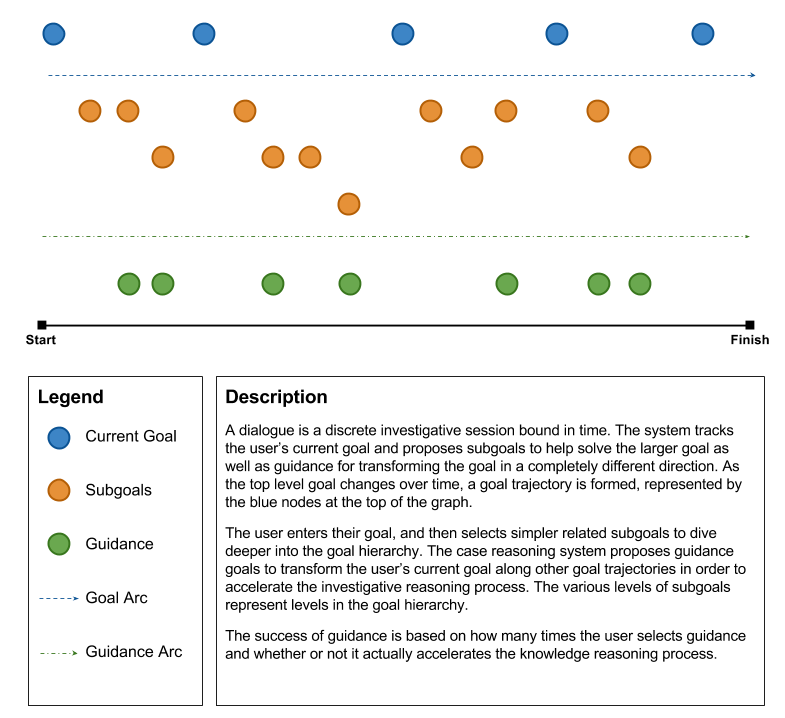
\includegraphics[width=\columnwidth]{figures/dialogue.png}
    \caption{A dialogue is a discrete investigative session that has an initial knowledge-goal and some different concluding knowledge-goal. By tracking goal changes throughout the dialogue, a reasoning system can construct the user's goal trajectory.}
    \label{fig:dialogue}
\end{figure}

In the context of an interactive knowledge-goal reasoning system that attempts to augment a user whose goals are changing throughout the investigation, a dialogue is a discrete investigative session. That is, in a dialogue a user provides an initial knowledge goal (represented as a natural language question) thus initiating the interactive dialogue. The system provides answers through traditional information retrieval techniques or by answering fact-based sub knowledge goals via a structured knowledge base. It also provides guidance in the form of new goals that may accelerate the goal change process towards a final goal or to prevent the user from pursuing fruitless paths of inquiry. During the dialogue the system tracks goal changes by recording when new, different knowledge goals are entered into the system. The dialogue is completed by a final knowledge-goal, which is presumably the target of the investigation.

By tracking goal changes and the knowledge-goals that proceeded them, a system can construct a goal trajectory from a dialogue. In fact, there is a one to one relationship between a dialogue and a goal trajectory. Since dialogues occur in context, e.g. at some time, in some location, on some device; cases can be adapted to the specific context of the user, which therefore improve guidance. It is for this reason that it is not correct to inspect or compare dialogues on their own, but rather to embed contextual information into the goal itself, so that similar goals may be proposed to the user. Dialogues are summarized in Figure \ref{fig:dialogue} as an ordered set of knowledge goals, sub-knowledge goals (e.g. simpler knowledge goals designed to add information to the top level goal) and guidances that cause goal change.

\section{Distance Based Guidance}

\begin{figure}
	\centering
    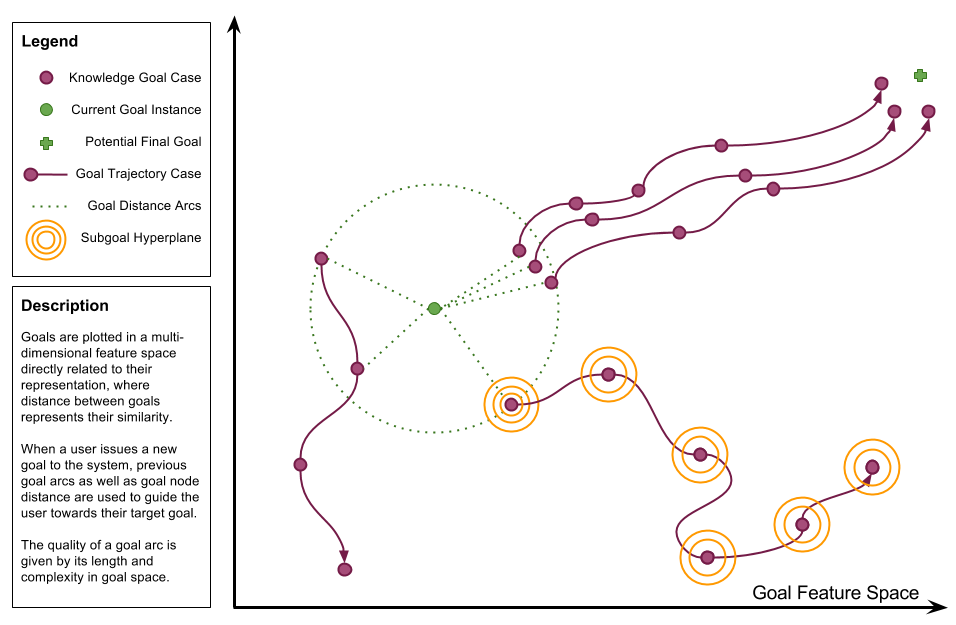
\includegraphics[width=\columnwidth]{figures/representation.png}
    \caption{A representation of the knowledge goal dimensional space. Each goal is a point in this space, and a trajectory is a path through knowledge goals. A user is accelerated if they can be guided to or through a similar goal trajectory, skipping over unnecessary goals. A user short-circuits dead ends or tangents in complex knowledge goals by maintaining a vector towards the final point in the followed trajectory.}
    \label{fig:representation}
\end{figure}

Distance based guidance requires the encoding of knowledge goals into a vector representation such that related or similar knowledge goals are close together in goal space. By computing the relative distances of knowledge goals in goal space, a goal trajectory can be said to have a length, that is the sum of the distances between the knowledge goals that compose the trajectory. The magnitude of the goal trajectory is the distance between the starting knowledge goal and the final knowledge goal.

If the length of the trajectory is much greater than its magnitude, then the user has followed a complex and circular path to their final goal. Part of the reason for this could be tangential or false starts down investigative paths. A \textit{short circuit} of a complex knowledge goal means that the guidance provided by the system brings the ratio of a goal trajectory's length and magnitude closer to 1 - preventing complexity or poor reasoning.

When the length is shorter than or equal to the magnitude of the goal trajectory, this indicates a straight forward line of investigation that proceeds in an ordered fashion directly towards the final goal. In cases like this, guidance will \textit{accelerate} the user towards the final goal, such that they may skip intermediate knowledge goals and arrive at their final goal much faster. However, here a system must be careful; it cannot simply point the user to the end of the goal trajectory as that might cause confusion when it is not clear how the path to that knowledge was deduced. Instead, acceleration skips over knowledge goals in the investigative chain, possibly providing feedback about why the acceleration would help. This feedback allows the user to more closely associate the reasoning path with the system's guidance and trust it.

Figure \ref{fig:representation} shows how guidance might be given for an initial knowledge goal. Given some goal, $G_{green}$, propose the $k$ closest goals such that the goal trajectory has the same or similar vector towards some final goal. Complex knowledge goals are not preferred and may be eliminated as proposals for guidance. Stochastic techniques may be used to help the user explore new investigative opportunities.

\subsection{Knowledge Goal Space}

The knowledge goal space is a dimensional representation of all possible knowledge goals where a point in this multi-demensional space is a knowledge goal. Similar knowledge goals should therefore be close together as measured by a geometric distance. The goal vector space is created by features of the natural language question that represent the \textit{concepts}, the \textit{context}, and the \textit{task} of the knowledge goal. In particular, each of these components of the knowledge goal representation is a unique vector that is unioned with the other three components to form the complete vector.

\begin{enumerate}
    \item \textbf{Concept Vector}: The concept vector uses a TF-IDF vector of the words in the natural language question. Because natural language questions are so short, TF-IDF is a good measure of the importance of infrequent words in the question corpus. Moreover, this vector is reduced by a truncated singular value decomposition (SVD) such that only the 50 best components of the vector remain.
    \item \textbf{Task Vector}: We have identified 9 potential task related to why the knowledge goal is being solved including factual questions like ``who'' or ``what'', explanation questions like ``why'' or ``how'', as well as existential and permission tasks. This vector is simply a boolean vector of the tasks of these questions based on a lightweight syntactic analysis.
    \item \textbf{Context Vector}: The context vector embeds user specific information into the goal including time of day, location of query, as well as relative position of the knowledge goal in a dialogue.
\end{enumerate}

These component vectors are easily computed from a natural language question using a lightweight parsing technique. The final knowledge goal representation is simply the ordered union of the concept, task, and context vectors. Because the TF-IDF vector in particular has to be computed on a medium to large corpus of questions ahead of computing the vector at run time, three corpora were used: \textit{Free917}, \textit{WebQuestiosn}, and \textit{Kyudo}. The distribution of questions from this corpus is shown using a principle component analysis (PCA) of the two most informative directions of each dimension, then mapped to two dimensions as shown in Figure \ref{fig:goalspace}.

\subsection{Neighbor-Based Guidance}

In order to provide guidance to the users, during a dialogue the current working knowledge goal was mapped to goal space, then a $k$-Nearest Neighbors algorithm was applied to filter the goals to potential candidates. The $k$ goals were suggested to the user, but were not ranked on distance alone but also the trajectory or initial of the goal in goal space from the proceeding goal. E.g. if a goal was in the ``same'' direction as the current path of the goal trajectory, then it would be prioritized even if it was a bit more far distant.

\section{Results}

\begin{figure}[!t]
	\centering
    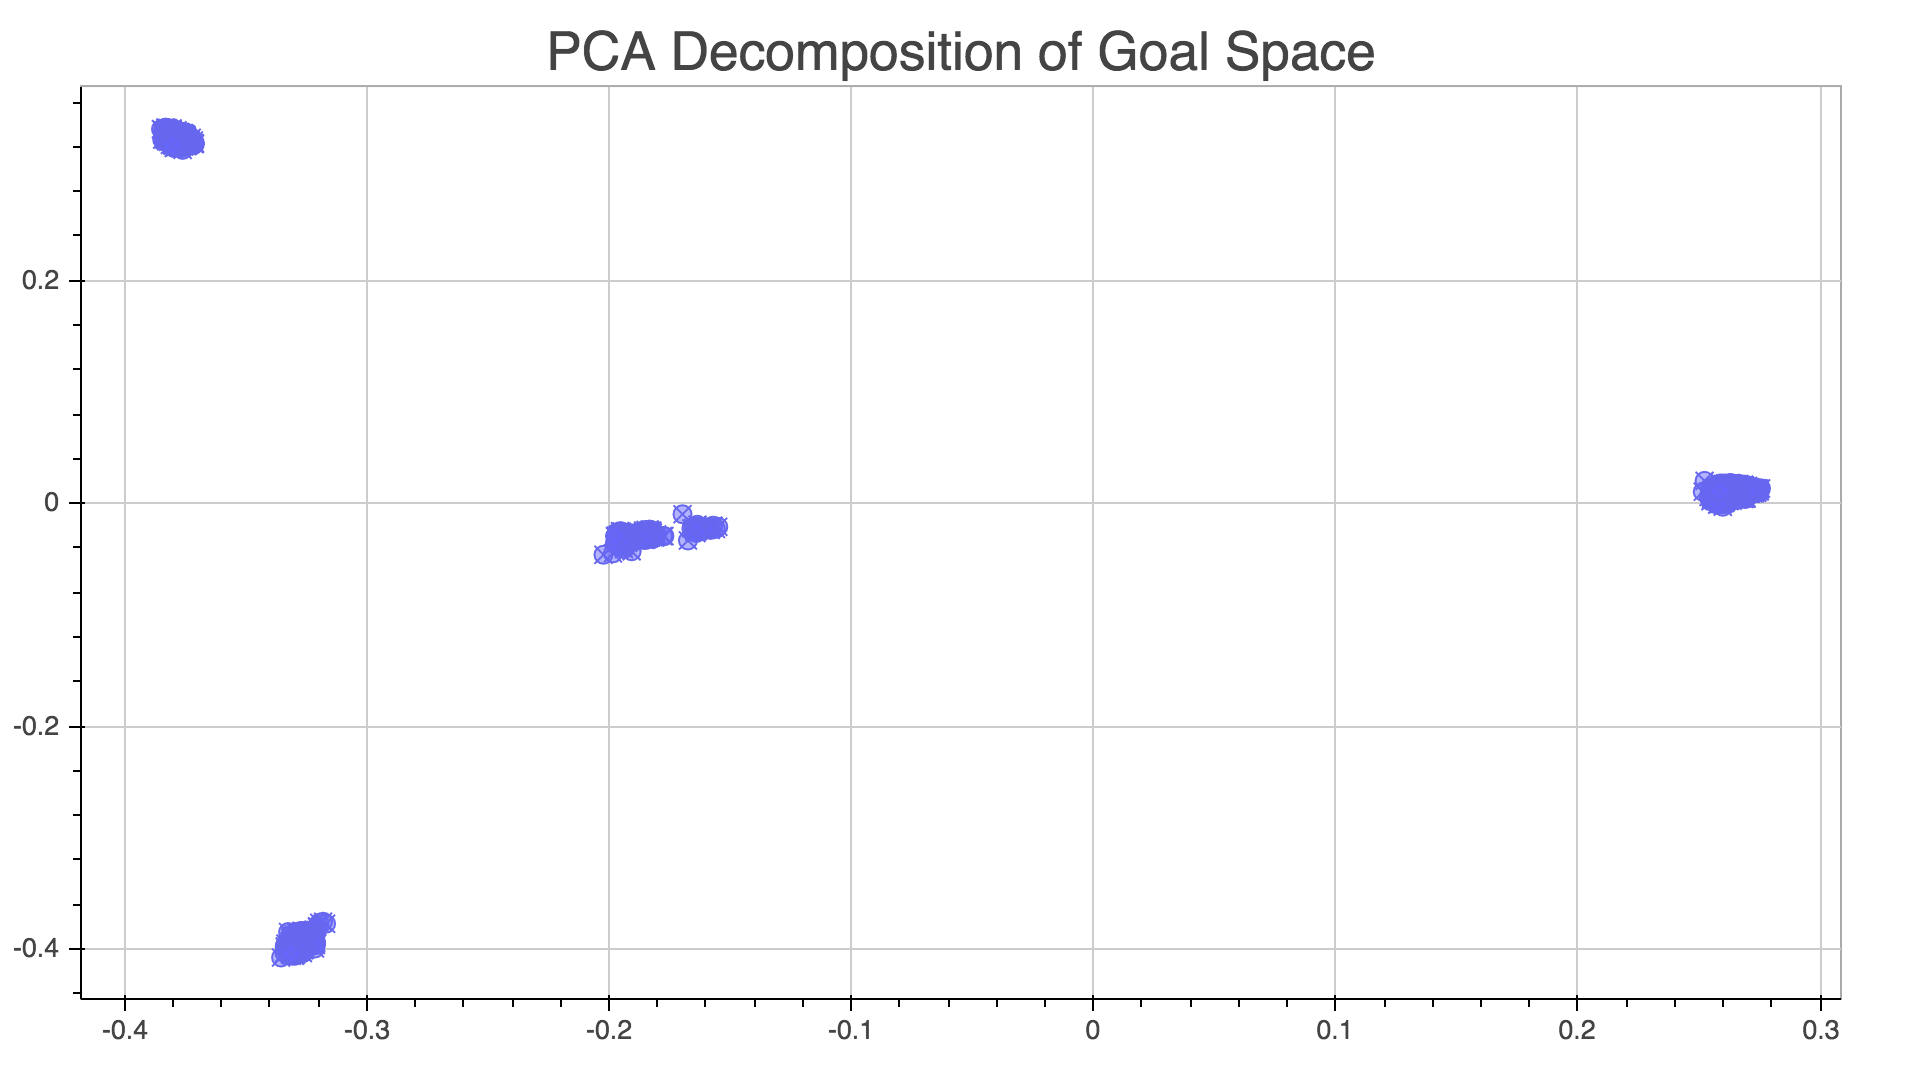
\includegraphics[width=\columnwidth]{figures/goalspace.png}
    \caption{PCA projection of knowledge goals from the \textit{Free917}, \textit{WebQuestions}, and \textit{Kyudo} corpus of knowledge goals. Note that 5 distinct clusters have formed, generally related to task.}
    \label{fig:goalspace}
\end{figure}

In order to test the results we replay observed dialogues and goal trajectories that were added to our system, but augmented with guidance. The augmentation creates a branching linear data structure of the goal trajectory, and we compute the minimum path distance from the initial goal to the final goal. Normalized by the percent of the minimum path that are guidance goals, we compute the short circuit or acceleration that guidance provides. Guidance is said to provide an improved goal trajectory if the ratio of the length and magnitude become closer to 1 for the case of short circuiting and in the case of acceleration, if the total number of nodes in the trajectory is fewer. 

\section{Conclusion}

No conclusion quite yet.

\bibliographystyle{aaai}
\bibliography{papers}

\end{document}
